\documentclass[10pt]{article}
\oddsidemargin -0.05in \topmargin -0.25in
\textwidth 6.5in \textheight 8.5in

\usepackage[english]{babel}
\usepackage{graphicx}
\usepackage[amssymb]{SIunits}% SI units package
\usepackage{color}
\usepackage{amsmath}
\usepackage{subcaption}
\renewcommand{\Re}{\mathrm{Re}}
\newcommand{\strong}[1]{\textbf{#1}}
\newcommand{\red}[1]{\textcolor{red}{#1}}
%\newcommand{\makered}[1]{\textbf{#1}}
\newcommand{\question}[1]{\begin{quote} \emph{#1}  \end{quote} }

\newcommand{\comm}[1]{}
\bibliographystyle{jasanum}


\begin{document}

\noindent Date: \today \\
Manuscript: IJMF\_2017\_854\\
Title: Air cavities at the inner cylinder of turbulent Taylor-Couette flow \\
Authors: Ruben A. Verschoof, Dennis Bakhuis, Pim A. Bullee, Sander G. Huisman, Chao Sun, Detlef Lohse

\vspace*{1.25cm}
\section*{Referee 2}
We thank the referee for her/his detailed comments and for his/her support to our work. We react to all comments below.

\question{The paper presents an experimental characterization of air cavities developed downstream cavitators attached at the inner cylinder wall of a Taylor Couette device in the turbulent regime. The context is drag reduction by ventilation for marine applications. \vspace{\baselineskip}\\
 The specificity of the device lies in the fact that it is a closed loop. Thus, to my best knowledge, it is the first time that ventilation downstream cavitators is studied in such a geometry. \vspace{\baselineskip}\\
The Taylor Couette device is the $T^3C$ facility characterized by a radius ratio of 0.716 and an aspect ratio of 11.7. The $T^3C$ device is well known for the accuracy of the viscous torque measurements it enables. \vspace{\baselineskip}\\
The cavitators are designed so that their axial dimension equals the inner cylinder height, their radial height is fixed, equal to 2mm (ie: 2.5\% of the gap width). Only one geometry of cavitators was studied in this paper, but 3 different arrangment were studied by varying the number of cavitators periodically spaced in the azimuthal direction (from 2 to 6 cavitators) \vspace{\baselineskip}\\
 Most of the results were obtained for the outer cylinder at rest but a case of counter-rotation was also investigated corresponding to a ratio of 0.2 between the rotational velocity of outer and inner cylinder. For the outer cylinder at rest, the Reynolds number is varied in the range [$10^5-10^6$]. For counter rotation, the Reynolds number is varied in the range [$10^5-1.5 \times10^6$]. \vspace{\baselineskip}\\
The air volume fraction available for entrapment in the cavity is controlled by the level of the free surface in the gap (free surface under the top of the inner cylinder). Most of the measurements have been completed for this procedure of ventilation for 2 different air volume fraction (2\% and 4\%).\vspace{\baselineskip}\\
But air injection can also be activated though the shaft and the cavitators. In this latter case, the air injection rate is controlled. \vspace{\baselineskip}\\
I have many questions about these procedures of ventilation in the cavity, particularly it is not clear for me how the authors really control the global void fraction inside the cavity when increasing the Reynolds number. See my following questions. \vspace{\baselineskip}\\
 Geometrical characteristics of the air cavity (streamwise length at different axial positions and global coverage of the inner cylinder) were obtained by visualisations and images processed manually. The sensitivity of these characteristics to the Reynolds number and to the air volume fraction available was analysed for the outer cylinder at rest. \vspace{\baselineskip}\\
 The viscous torque applied on the inner cylinder was measured for the different flow conditions (different Reynolds numbers, inner cylinder at rest or counter rotation, different arrangement of cavitators, different values of air volume fraction available 2\% and 4\%, with and without air injection through the cavitators). The torque measured is compared to the one obtained in the single phase flow with the cavitators, thus leading to a gross relative variation of the torque (air cavity induced variation). Comparison of the torque measured is also made with the one obtained in the single phase flow without the cavitators, thus leading to a net relative variation of the torque (air cavity and cavitators induced variation). This approach is particularly interesting as it takes into account the increase in the torque due to the addition of the cavitators. \vspace{\baselineskip}\\
 Based on the results,  this paper gives a first evidence of the existence and sustainability of air cavities in a Taylor Couette flow. The observed gross drag reduction is clearly linked to the air cavity coverage of the inner cylinder, which might be optimal for some specific design of the cavitators. Interesting enough is : \vspace{\baselineskip}\\
1)     - the observation of a saturation of the air cavity length, global air coverage and gross drag reduction for high Reynolds number.\\
2)     - The demonstration that air injection through the cavitators is not necessary to generate and sustain the air cavity in this closed loop. Moreover, for the air injection rate at stake, the gross drag reduction doesn't depend on the air injection rate but rather on the available air volume fraction above the free surface. I have questions and particular remarks about this results (see in the following)\\
3)      -The demonstration that with the addition of the cavitators, there is a net drag increase, while air cavity occurrence induces a gross drag decrease. \vspace{\baselineskip}\\
As a conclusion, this paper provides an interesting experimental investigation of a 2 phase flow that was not studied before. The paper is very clear, well written and well organized. There is also a good overview of the literature. The measurements are achieved with caution and the results look reliable. I'm keen to accept it. However, there are a few points which I would like the authors to address before the paper can be actually accepted (some of them are major points) : \\
            -Complete the description of the measuring system\\
            -Discuss the procedure which consists of controlling the air volume fraction\\
            -Evaluate the impact of the change in wetted height of the inner cylinder on the value of gross drag reduction\\
            -discuss the relationship between gross drag reduction and air cavities coverage\\
            -further discuss the evolution of the cavity length, with regards to the Reynolds number\\
            -further discuss the contribution of air injection through the cavitator by defining a non dimensional parameter (volumetric fraction) that can be compared to void fraction available above the free surface\\
            -add other non dimensional parameters for comparison to air cavities in channel flow (cavitation number ?) \vspace{\baselineskip}\\
All these points that should be clarified are detailed below.}

\noindent \strong{1a}

\question{\underline{Description of the measuring system} \\
-Description of the visualization system is uncomplete. \\
Add the scale or the field of view, add the frame rate and describe the lightning system. Indeed, the lightning system is here an important parameter to have images, not saturated but with a good contrast, fitted to image processing. I understand that images have been processed manually (it is not a reproach, I can understand the difficulty of analyzing such kind of images)  but how you proceed for the light must be described.
 }

\noindent \strong{Response:} 

\noindent We now added additional explanation in the method section. One particular difficulty in TC flow is the presence of the curved cylinders. These make a homogeneous light intensity very difficult. Therefore, we now improved our figures by means of digital processing. The camera settings: we used a shutter speed of 1/5041 s for the images in figure 4 and a shutter speed of 1/16000 s for figure 5. We used the same lens and camera for all measurements, and thus the field of view angle was 23$^{\circ}$ for all cases.\\
	 
\noindent \strong{1b}

\question{What was the measurement time (related to time periods of the TC two phase flow), what was the number of images, what was the number of air cavities, taken into account for statistical characterization (cavity length and coverage)? Was there a periodic break off of the cavity by the re-entrant jet, if so what was the value of this frequency and does the measurement time consider this aspect?
 }

\noindent \strong{Response:} 

\noindent As the referee mentioned in comment 1a, indeed, all images are processed manually. Therefore, we tried to find a method which is both accurate and easy-to-use. We now averaged 100 independent instantaneous photos of air cavities over 33 consecutive rotations, which results in 1 averaged figure. In these 100 images, all parameters, as well as the angular position of the cavitator was the same. In this way, we reduced the influence of air cavity length fluctuations.\\
About the re-entrant jet: as the cavity itself moves together with the inner cylinder, it leaves the field-of-view within a number of frames. therefore, we are unable to extract any frequency of the periodic break off.\\
We now added this to our manuscript. \\

\noindent \strong{1c}

\question{In Fig.6 and 7., the authors say they show estimated error bars. I don't see them on these figures. So please, could the authors add the error bars due to statistical convergence on the figures?
 }

\noindent \strong{Response:} 

\noindent Rather than showing individual error bars on every single datapoint, we chose to include 1 errorbar for the figure as a whole. This errorbar was already included in the figures of the original manuscript. We now made its position clearer in the caption.\\

\noindent \strong{1d}

\question{The authors should remind the accuracy of the torque measurement system (even if it is given in details in Van Gils (2011)). They should evaluate the accuracy they have for the determination of the normalized torque G, when correction is made with the viscosity of the liquid at a measured temperature. Evaluate the accuracy for the determination of DR (\%). Add error bars when DR is displayed (figures 8b), 9b, 10b), 11b)) }

\noindent \strong{Response:} 

\noindent In the revised manuscript, we added errorbars to all figures showing torque and DR data.\\

\noindent \strong{2a}

\question{\underline{Control of air volume fraction}\\
I don't understand how the authors control the air volume fraction $\alpha$ of the device, without injection.\\
Is a measured at rest? Is it just based on the measurement of the liquid height, and air gap height above the free surface, at rest? If so, $\alpha$ is an initial value of the void fraction, it just represent the total amount of air volume fraction available, but it doesn't mean that this is the real air volume fraction entrapped. If so, I suggest that the authors precise that $\alpha$ is the air volume fraction available in the device above the free surface, and characterized at rest.
 }

\noindent \strong{Response:} 

\noindent The void fraction is measured at rest, and indeed, it is the amount of available air rather than the effective, or real void fraction at any given position. In fact, there will never be a uniform effective void fraction, due to buoyancy and centrifugal forces, as was shown in  \cite{gil13}.   \\
We follow the referees suggestion, and now added the notion that the void fraction is measured at rest.\\

\noindent \strong{2b}

\question{Based on this remark, I don't agree with the authors when they evaluate the equivalent thickness of the cavity, based on the cavity coverage and the value of imposed $\alpha$. Indeed, the real void fraction will be different, thus leading to different value of the thickness of the cavity than 8mm.
 }

\noindent \strong{Response:} 

\noindent This cavity thickness value is an estimation. We assume that all air is attached to the cavity, as is stated in the accompanying text. \\

\noindent \strong{2c}

\question{With the increase of the Reynolds number (or inner cylinder velocity), the air entrapment through the free surface increases (without and with cavitators). Thus, one expect the level of the free surface to rise up. So I don't see how you can control the air volume fraction, for different Reynolds number, the real void fraction will be different.
 }

\noindent \strong{Response:} 

\noindent The amount of water in the setup (with a volume fraction of $1-\alpha$) is constant both in mass as in volume, as the temperature is kept constant. Consequently, the volume percentage of air in the setup cannot change during the measurements. But indeed, in line with our response on comment 2a, the effective void fraction in the flow depends on the axial and radial position, and then also varies with Reynolds number. \\
We now added this notion to our revised manuscript. \\

\noindent \strong{2d}

\question{Maybe, it should be interesting to measure the localization of the free surface (and thus deduce a real void fraction), when increasing the Reynolds number, but I suppose it is difficult since the free surface is not plane and is submitted to instabilities (consider it as a comment, not mandatory).
 }

\noindent \strong{Response:} 

\noindent As the referee already suggests: the free surface is horizontal only without inner cylinder rotation. Even at the smallest achievable rotations, the free surface becomes first curved, and later unstable. Eventually, it disappears completely, once the liquid is pressed against the upper plate. Therefore it is too difficult to measure its location, and in general not meaningful to measure the height of the free surface. For the presented torque data there is no free surface anymore; all the air is entrained in the flow.\\

\noindent \strong{2e}

\question{Except figure 12, at the end of the paper, all the results are shown for the procedure which consists of imposing the available air volume fraction, without injection though the cavitator. This must be clearly specified in the text and in the title of all these figures (from fig. 4 to fig. 11). Indeed this is only specified at the end of the paper in p. 16 ('In all measurements presented above, we did not inject air locally, but instead chose to fill the cylinder only partially'), it is too late, it must be mentioned much earlier in the paper, otherwise the reader raises the question of the protocol used.
 }

\noindent \strong{Response:} 

\noindent We agree with the referee, and we now added this notion to the method section, to avoid any misunderstandings.\\

\noindent \strong{3a}

\question{\underline{Height of the inner cylinder wetted and impact on $G$} \\
For the protocol which consists of imposing a partial filling of the gap width, with a control height of the free surface, I don't understand why the authors don't use the real wetted height l of the inner cylinder to calculate the normalized torque $G$, rather than $L$, which is the entire height of the inner cylinder. }

\noindent \strong{Response:} 

\noindent Even at low rotation rates, the free surface disappears completely, as all air is entrained in the bulk flow as bubbles or as an air layer behind a cavitator. Some snapshots of the flow are provided in figure 4 of the original manuscript, in which no free surface is shown. As the free surface already is absent at the lowest Reynolds numbers we measure, we consequently use $L_{IC}$ to non-dimensionalize our torque. We refer the referee to our response to comment 14. Indeed, there is a difference between $L$ --- the height of the setup, and $L_{IC}$ --- the height of the inner cylinder. We consequently non-dimensionalize our torque with $L_{IC}$.\\

\noindent \strong{3b}

\question{Indeed, $l=(1-\alpha)L$ will be different than the case of single phase flow. For a=2\% and 4\%, this correction of the height leads to a relative increase of G from 2\% and 4\% respectively. This will reduce the obtained value of gross drag reduction?
 }

\noindent \strong{Response:} 

\noindent With cylinder rotation the `free surface' disappears, as air is entrained due to turbulent mixing and centrifugal forces. Therefore, we normalize $G$ with $L_{IC}$ rather than with $L_{IC}(1-\alpha)$. For more explanation, we refer the referee to our response to comment 3a. \\

\noindent \strong{3c}

\question{Also, the height $l=(1-\alpha)L$ could be used when the air cavity coverage is determined (total area between 2 cavitators$=2\pi r_i L/3)$.\\
 I agree it will not change the qualitative trends observed and comments of the paper, but it can modify the measured quantities a little.
 }

\noindent \strong{Response:} 

\noindent The free surface disappears completely. We chose to stick to the use of $L_{IC}$ for the calculation of the coverage. For more explanation, we refer the referee to our response to comment 3a and 3b. \\


\begin{figure}[htp]
\begin{center}
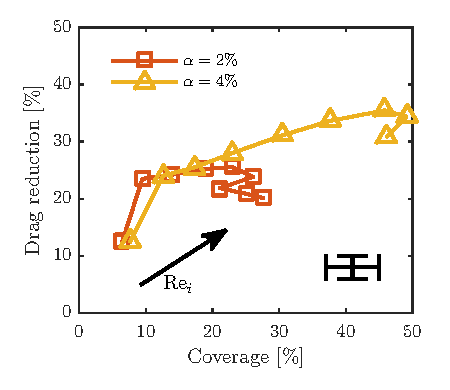
\includegraphics[scale=1]{ref2_DR_cov.eps}
\caption{Drag reduction as a function of air coverage for global void fractions of $2\%$ and $4\%$.} 
\label{DR_cov}
\end{center}
\end{figure} 

\noindent \strong{4}

\question{\underline{Relationship between gross drag  reduction and air coverage of the inner cylinder} \\
For the outer cylinder at rest, and Reynolds numbers for which the authors have characterized the geometry of the cavity by image processing, could the authors add a graphics where the gross drag reduction is plotted versus the air cavity's coverage, using different colors or symbols for alpha=2\% and alpha=4\%, and comments? }

\noindent \strong{Response:} 

\noindent We thank the referee for this suggestion, and we show the result in figure \ref{DR_cov}. We agree with the referee that this figure is useful, and we now show it in the revised manuscript.\\

\noindent \strong{5a}

\question{\underline{Analysis of the cavity length when varying the Reynolds number} \\
First of all, the authors should add in Fig.\ 6, the streamwise distance between two neighboring cavitators, as this distance is a limit for streamwise length of air cavity.
 }

\noindent \strong{Response:} 

\noindent We now added this distance to the figure as well as to its caption. Furthermore, we now normalized the cavity length with the cavitator distance on the right y-axis.\\

\noindent \strong{5b}

\question{I don't understand why axial stratification of the cavity length is more pronounced when the Reynolds number increases. It should decrease as the inner cylinder velocity increases, making the ratio of buoyancy force to inertia force decreasing. Could the author had a comment on this aspect. }

\noindent \strong{Response:} 

\noindent The axial stratification only fully disappears at even larger rotation rates. In ref.\ \cite{gil13}, van Gils et al.\ measured the local void fraction in the same experimental setup at $\Re_i = 1\times 10^6$, i.e.\ the same Reynolds number we achieve here. It was found that also at these Reynolds numbers the axial dependence of local void fraction is significant. Due to a number of experimental difficulties, we currently cannot rotate at higher rotation rates. Only for $\Re_i \to \infty$ we can fully neglect buoyancy forces.\\


\begin{figure}[htp]
\begin{center}
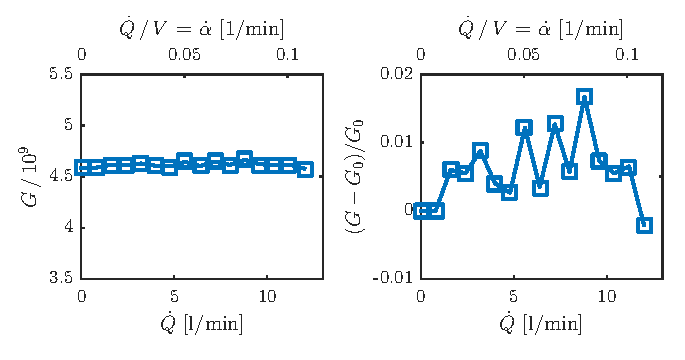
\includegraphics[scale=1.1]{fig12_new.eps}
\caption{Influence of the air injection rate on the torque. Now, we show in (a) the absolute value of the dimensionless torque $G$, and in (b) the relative change in torque, in which $G_0 = G(Q=0)$. The Reynolds number is $Re_i = 1 \times 10^6$, and the global void fraction equals $\alpha = 2\%$.} 
\label{inject_new}
\end{center}
\end{figure} 

\noindent \strong{6a}

\question{\underline{Discussion about the contribution of Q (air injection through cavitators)} \\
First of all, before concluding that Q has quite no effect on gross Drag reduction, rather plot in figure 12, the relative variation of G as DG/G(Q=0). If it is confirmed to be very small by comparison to gross drag reduction (ie: 20\%) achieved at this Reynolds number for alpha=2\%, then you can conclude that air injection though the cavitaton, has no influence, but for this range of air injection
 }

\noindent \strong{Response:} 

\noindent We agree with the referee that such a plot is useful, see fig.\ \ref{inject_new}. We now added it to our manuscript. We also added the notion that for this range of air injection the influence is negligible.\\

\noindent \strong{6b}

\question{In Fig. 12, the authors should plot the relative variation of $G$, with regard to $Q/V/\omega_i$ ( in \%) rather than $Q/V$ (in 1/min). With $\omega_i$ being the rotational velocity of the inner cylinder (tr/min), $Q/V/\omega_i$ is a non dimensional parameter, representative of a volumetric fraction of the air injected through the gap.
 }

\noindent \strong{Response:} 
\begin{figure}[htp]
\begin{center}
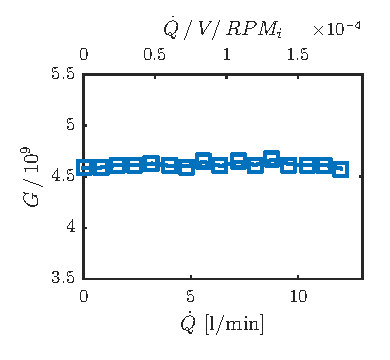
\includegraphics[scale=1.1]{fig12_ref.eps}
\caption{Influence of the air injection rate on the torque. The top x-axis is now non-dimensialized as $\dot{Q}/V/RPM_i$, in which $RPM_i$ equals 600 RPM. The Reynolds number is $Re_i = 1 \times 10^6$, and the global void fraction equals $\alpha = 2\%$.} 
\label{fig:inject}
\end{center}
\end{figure} 
\noindent We provide the requested plot in figure \ref{fig:inject}. The authors were also struggling with ways to really non-dimensialize the air injection rate, and using $\omega_i$ (here having as RPM as dimension) was one of the options we had considered. However,  the timescales in $Q$ and $\omega_i$ are not related. Therefore, we think that non-dimensializing $Q$ using $\omega_i$ is not valuable. Therefore, we chose to leave the figure as it was.\\


\noindent \strong{6c}

\question{This volumetric fraction of air injected can be directly compared to the void fraction available above the free surface alpha. If it is very small, compared to $\alpha$, this attests for the negligible influence of air injection through the cavitators, for the range of air injection rate of the study. }

\noindent \strong{Response:} 

\noindent We agree with the referee, that if the amount of injected air is small compared to $\alpha$, the air injection can be expected a priori to be useless. This is not the case in our work. In the figure we show, the global void fraction is $2\%$, corresponding to 2.2 liters. We inject up to 12 liters per minute, which is a significant amount compared to the amount of air inside the experimental setup. \\
We now highlight this notion in the revised manuscript.\\
\\


\noindent \strong{7a}

\question{\underline{Non dimensional parameters} \\
In table 1, also add the parameter $Q/V/\omega_i$, this parameter will contribute in the limit of very high $Q$ or low Re (which is not tested here)
 }

\noindent \strong{Response:} 

\noindent We refer the referee to our response to comment 6b. As we the timescales in $Q$ and $\omega_i$ are unrelated, we think that plotting the quantity $Q/V/\omega_i$ does not result in additional insight or understanding. Therefore, we chose not to include this parameter in table 1.\\

\noindent \strong{7b}

\question{When comparison is made between the TC flow and the channel flow, parameters $\sigma_v$ and $\sigma$ are missing (cavitation parameter). Indeed, it is necessary to quantify the natural cavitation. In TC flow, it implies the low pressure in the cavity (PC) to be known. Maybe it can be a-priori estimated based on the height of the cavitator $h$, and the azimuthal velocity of the inner cylinder $u_i$.
}

\noindent \strong{Response:} 

\noindent Indeed, these dimensionless numbers are commonly used in channel flow. In our setup it is not possible to measure the local pressure in the cavity. Furthermore, the pressure in the setup varies with the height: a difference of almost 0.1 bar in between the top and the bottom. Therefore, even if we would be able to measure the local pressure, $\sigma$ would not be a constant parameter.
However, the notion of the cavitation parameter adds to the comparison between channel and TC flow, and we now added it in the table for comparison. We defined $\sigma_{TC}$ as $(p(z) - p_c) / (\frac12 \rho u_{\infty}^2)$, in which $p_c$ is the pressure in the cavity and $p(z)$ is the height-dependent free stream pressure. \\

\noindent \strong{Minor points: 8}

\question{In the summary, the authors say : ``to study the effect and dynamics of air cavities in this closed setup''. I don't see where in the paper, the authors study the dynamics of the air cavity, so please suppress ``dynamics'' in this sentence'
 }

\noindent \strong{Response:} 

\noindent We rewrote this sentence, to avoid this minor misunderstanding.\\

\noindent \strong{9}

\question{Highlights: In the sentence : `Local air injection does not change the drag reduction, as long as void fraction is constant', I don't understand the meaning of `as long as void fraction is constant'. Could the authors reformulate this sentence?
}

\noindent \strong{Response:} 

\noindent We agree with the referee that this sentence can be improved. We now changed it to: ``Local air injection is not crucial for efficient drag reduction --- as long as sufficient air is available anywhere in the flow.''\\

\noindent \strong{10}

\question{Literature survey: In the introduction, in page 4, Rosenberg et al. (2016), Saranadhi et al. (2016), Srinivasan et al. (2015) are included in the studies of bubbly drag reduction. Please, get rid of them in this part, as they rather deal with hydrophobic surfaces and air layer drag reduction. They are correctly cited at the top of p5 when the issue of air layer is addressed. \\
In p. 13, when the authors explain the decrease in gross drag reduction for counter rotating inner cylinder by the entrapment of bubbles in the turbulent Taylor vortices, the authors could refer to Fokoua et al. (2015). This author evidenced for the bubbly Taylor Couette flow that preferential entrapment of the bubbles in the Taylor vortices rather increases the viscous torque, and the contrary for preferential entrapment near the inner cylinder. }

\noindent \strong{Response:} 

\noindent The referee is right: indeed, strictly speaking the referenced works do not study \emph{bubble} drag reduction. We now omitted these from this part of the introduction. \\
On the suggestion to add a reference to Fokoua et al.: this article studies a completely different Reynolds number regime, i.e.\ $600 \leq Re_i \leq 2\times 10^4$. Therefore, the physical mechanisms of drag reduction are different: in this regime the buoyancy forces are more dominant, and the flow is not yet fully turbulent. We now added this reference in the introduction.\\

\noindent \strong{11}

\question{Outline at the end of the introduction: In the description of the outline, part II.B is not introduced }

\noindent \strong{Response:} 

\noindent We thank the referee for pointing this out. We now added the introduction of part IIB. \\

\noindent \strong{12}

\question{In fig. 1 (b), the position of the torque sensor is not clear for me. Also, if $L$ is the height of the inner cylinder, the row denoting $\alpha L$ must not reach the top of the device, but reach the top of the inner cylinder }

\noindent \strong{Response:} 

\noindent We thank the referee for pointing this out. $L$ is the height of the outer cylinder, which is slightly larger than the height of the inner cylinder, to which we now refer as $L_{IC}$. We now changed our experimental method section accordingly. In figure 1b, we added a sentence to better explain the torque sensor position.\\






	\bibliography{literatur,2ph_literatur}


\end{document}